%% ====== Classe du document ============================================
\documentclass[10pt,a4paper]{report}
\usepackage[left=1.5cm,right=1.5cm,top=2cm,bottom=2cm]{geometry}

%% ====== Francisation ==================================================
\usepackage[french]{babel}
\usepackage[T1]{fontenc}
\usepackage[utf8]{inputenc}
\usepackage{textcomp}

%% ====== Personnalisation ============================================
\usepackage{fancyhdr}
	\lhead{}
	\chead{Acquisition et analyse d'image}
	\rhead{M2 IGI 2013-2014}
	\renewcommand{\headrulewidth}{0.3pt}
	\renewcommand{\footrulewidth}{0.3pt}
	\lfoot {hadrien.croubois@ens-lyon.fr}
	\cfoot {- \thepage -}
	\rfoot {}
	\pagestyle{fancy}
\title{Acquisition et analyse d'image}
\author{Hadrien Croubois \and Nicolas Lourdeau}
\date{}

%% ====== Packages pour le texte ========================================
\usepackage{soul}
\usepackage[normalem]{ulem}
\usepackage{fancybox}
\usepackage{moreverb}
\usepackage[table]{xcolor}
%% ====== Packages pour les dessins =====================================
\usepackage{graphicx}
\usepackage{multicol}
\usepackage{multirow}
\usepackage{tikz}
\usepackage{lmodern}
\usepackage{pict2e}

%% ====== Packages pour les maths =======================================
\usepackage{amsmath}
\usepackage{amssymb}
\usepackage{mathrsfs}
\usepackage{bussproofs}
%%\usepackage[ruled,vlined,french]{algorithm2e}
%%\usepackage[squaren,Gray]{SIunits}


%% ====== Reglages generaux =============================================

\usepackage{titlesec}
	\titleformat{\section}[frame]
	{\normalfont}
	{\filright
	\footnotesize
	\enspace Partie \thesection\enspace}
	{6pt}
	{\bfseries\filcenter}
	
	\titleformat{\subsection}[frame]
	{\normalfont}
	{\filright
	\footnotesize
	\enspace \thesubsection\enspace}
	{6pt}
	{\filcenter}
%	{\titlerule
%	\vspace{.8ex}%
%	\normalfont\itshape}
%	{\thesubsection.}{.5em}{}

	\titleformat{\subsubsection}
	{\titlerule
	\vspace{.8ex}%
	\normalfont\itshape}
	{}{.5em}{}

\titleformat{\chapter}[display]
	{\normalfont\bfseries\filcenter}
	{}
	{1ex}
	{\titlerule[2pt]
	\vspace{2ex}%
	\LARGE}
	[\vspace{1ex}%
	{\titlerule[2pt]}]
	
\parindent=10pt

\usepackage{makeidx}
\makeindex
\newcommand\vect{\overrightarrow}

\numberwithin{equation}{subsection}


\graphicspath{{img/}}

\usepackage{subfigure}
\usepackage{hyperref}
\usepackage{draftwatermark}

%% ======================================================================
\begin{document}
\maketitle
%% ======================================================================
%% ======================================================================

\section{Philosophie d'utilisation}
Dans le cadre de ce projet, les outils développés ont toujours été prévu pour être réutilisés. Ainsi le code se décompose tout naturellement en deux parties, d'un coté une librairie facilement compilable au format \texttt{.so} ou \texttt{.dll} fournit avec les fichiers en-tête correspondant et d'autre part un programme simple appelant les fonctionnalités de la bibliothèque.

Afin de donner différents exemples d'utilisation de la bibliothèque \emph{lenactions}, deux applications sont fournies et donnent ainsi différents exemples d'utilisation plus ou moins haut niveaux des fonctionnalités de la bibliothèque.
\begin{itemize}
	\item \textbf{Lenaction} : programme simple, effectuant des appels à la bibliothèque à partir des arguments codés en dur dans le programme.
	\item \textbf{LenaSH} : un shell minimaliste interprétant des commandes écrites dans un langage ad-hoc et proposant ainsi une interface haut niveau pour l'utilisateur.
\end{itemize}

\section{Outils utlisés}
Afin d'optimiser la portabilité de la bibliothèque, cette dernière ne dépend d'aucun autre outil. Ecrite en C/C++ elle gère toutes les étapes du traitement d'images, du chargement de fichier au calcul de contours, en passant par la transition dynamique entre les espaces de couleur \textsc{rgb} et \textsc{hsv}.

Le programme \textbf{LenaSH} utilise les outils \textsc{flex} et \textsc{bison} pour la reconnaissance du langage ad-hoc développé parallèlement à la librairie.

Afin de simplifier l'étape de compilation des différents composants du programme sur différentes architectures, nous utilisons l'outil \textsc{CMake} ainsi qu'un script \texttt{./generator}.


\section{Fonctionnalités}

De nombreux algorithmes sont actuellement déployés dans la bibliothèque à différents niveaux :

\begin{itemize}
	\item Pixel :
		\begin{itemize}
			\item Conversion d'espace de couleur
			\item Opérateurs de fusion (quadratique, angle)
		\end{itemize}
	\item Image :
		\begin{itemize}
			\item Chargement/Sauvegarde au format \texttt{.ppm} / \texttt{.pgm}
			\item Calcul de seuil
			\item Composition avec un filtre
			\item Assemblage de deux images
			\item Seuillage (local, global, histerisis)
			\item Affinage de contour
			\item Calcul de contour fermés (méthode naive et méthode par vagues)
		\end{itemize}
\end{itemize}

La mise en place de filtre de convolution standard permet par ailleurs de calculer simplement les contours via les filtres de Prewitt, Sobel et Kirsch ainsi que d'appliquer un filtre moyenneur gaussien pour lisser l'image.



\section{Algorithme}
\subsection{seuillage par histerisis}
Cette opération de seuillage revient à calculer des composantes connexes pour le critère de luminosité $(>low)$ dans l'image. Pour cela on utilise une structure de \emph{union find} qui garantit un résultat rapide $\mathcal O(n.Ack^{-1}(n))$.

L'ajout d'un drapeau au niveau des composantes connexes permet de marquer les composantes dont un des éléments vérifie le critère de luminosité $(>high)$.

On ne garde ensuite que les pixels appartenant à une composante connexe marquée.

\subsection{Affinage des contours}
Pour cette opération, on se base sur une image de contour obtenue à partir de l'opérateur de mélange \texttt{angle} appliqué à deux gradients.

L'angle décrivant localement le contour (azimut du gradient) est discrétisé et permet de parcourir localement la largeur du contour. En ne gardant que le pixel au centre de ce contour on arrive à garder un contour fidèle, peu bruité et limitant les trous.


\subsection{Fermeture des contours}
\subsubsection{Méthode naïve}

Le première version développe est une méthode naïve se basant sur une vision purement locale du problème.

L'idée est de commencer par détecter, dans le contour affiné, les points caractéristiques de la discontinuité et de reconstruire les contours à partir de ces derniers.

Pour cela on effectue une marche qui consiste à partir du point caractéristique et à se déplacer de proche en proche en choisissant toujours d'aller vers le pixel voisin (en excluant le pas précédant dans la marche) qui présente la norme du gradient la plus importante (avant seuillage).

Les résultats sont intéressants sur des images simples avec des trous de petite tailles mais il nous est vite apparu que la vision local adopté par cette méthode n'est pas idéale pour résoudre une problématique globale. Nous avons donc cherché à mettre en œuvre une méthode plus complète.


\subsubsection{Méthode à vagues / par diffusion}

Cette variante est un algorithme inspiré des methodes de diffusion et des algorithmes à vagues utilisés en système distribué pour la communication sur des grilles de processeurs.

Ici chaque pixel est une entité pouvant être dans l'un des quatre états suivants :
\begin{itemize}
	\item \emph{Vide}
	\item \emph{Champ}
	\item \emph{Contour}
	\item \emph{Ancre}
\end{itemize}

Au début de l'algorithme, on part d'un contour affiné dont les pixels sont dans l'état \emph{Contour} tandis que le fond est dans l'état \emph{Vide}.

La première passe se charge de détecter les \emph{Ancres} parmi les pixels du Contour. Pour cela on détecte tout ceux qui ont soit aucun voisin (ancres d'adjacence 2) soit ceux qui sont en bord de contour (un unique voisin ou deux voisins collés) qui sont des ancres d'adjacence 1.

Les ancres sont les points d'intérêt qu'il s'agit de relier. Leur adjacence correspond au nombre de liaison à former pour faire partie d'un contour fermé.

A partir de là, on applique un algorithme de diffusion pour répandre un champ autour des ancres. Les pixels passent ainsi de l'état \emph{Vide} à l'état \emph{Champ}.

La jonction de champs provoque la liaison des deux ancres et la diminution de leur adjacence.

Si un champ rencontre un pixel d'un contour et que celui ci n'est pas dans la composante connexe de l'ancre associé au champ, il s'y accroche, faisant par la même occasion diminuer l'adjacence de l'ancre dont il provient.

Pour cette diffusion on utilise une file de priorité implémentée à partir d'un tas et une distance basé sur \textsc{BLUE} (best linear unbiased evaluation) qui prend aussi en compte les variations successives du gradient le long du contour à retrouver.

Cet algorithme donne de bons résultats des lors que la taille des trous est inférieure à la taille des composantes connexes à fermer. 

Voir la partie~\ref{resultats} (page~\pageref{resultats}).

\section{Conclusion}

Âpres de longue séances de recherche, nous sommes satisfait de la forme que prend notre bibliothèque. De nombreux outils précédemment développés dans le cadre de \texttt{LibImAMXX} (librairie graphique développé par Hadrien Croubois en M1 et qui a servi de support) sont actuellement en cours d'ajout. Parmi ces outils on compte notamment l'affichage des histogrammes avec \texttt{gnuplot}, la normalisation des espaces de couleurs ainsi que le tatouage.

Pour ce qui est des algorithmes développés, nous sommes relativement content des résultats renvoyés par l'algorithme d'affinage.

L'utilisation de champs dans un algorithme à vagues nous semble une piste intéressante pour la fermeture des contours. Beaucoup de travail reste cependant à faire, aussi bien pour ce qui est du choix de la fonction de distance que pour les heuristiques de création des liens d'ancrage.
Nous espérons pouvoir continuer à améliorer notre algorithme afin de le rendre plus efficace, notamment en s'adaptant dynamiquement aux propriétés de l'image.

Le code du programme est disponible sous licence GNU GPL v3 sur GitHub : \url{https://github.com/Amxx/Lenactions}

\appendix
\newpage
\section{Annexes - Résultats} \label{resultats}


\begin{figure}[ht]
	\center
	\subfigure[Formes géométriques]	{ 
\includegraphics[width=5cm]{imgs/test_image.png} }
	\subfigure[Lena]								{ 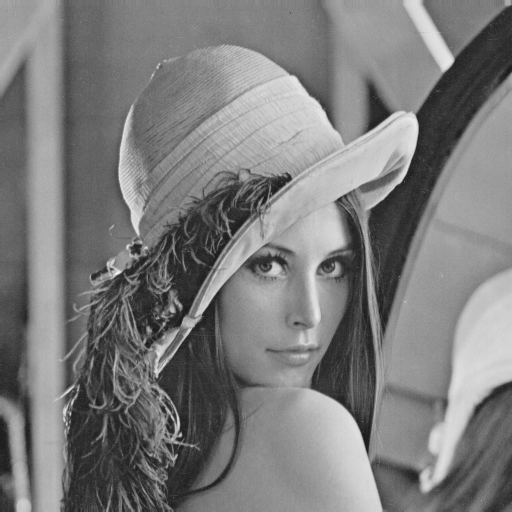
\includegraphics[width=5cm]{imgs/lena512.png} }
	\caption{Images utilisées lors des tests}
\end{figure}

\begin{figure}[ht]
	\center
	\subfigure[Gradient horizontal]	{ 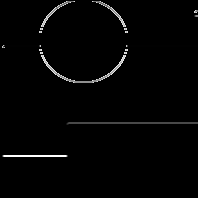
\includegraphics[width=5cm]{imgs/test/1a_hGrad.png} }
	\subfigure[Gradient vertical]		{ 
\includegraphics[width=5cm]{imgs/test/1b_vGrad.png} }
	\subfigure[Gradient composé]		{ 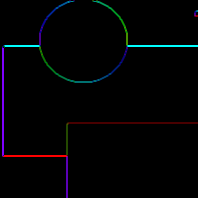
\includegraphics[width=5cm]{imgs/test/2_gTone.png} }
	\subfigure[Contour seuillé]			{ 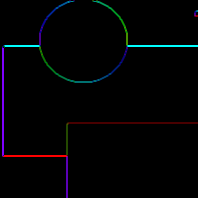
\includegraphics[width=5cm]{imgs/test/3_Border.png} }	
	\subfigure[Contour affiné]			{ 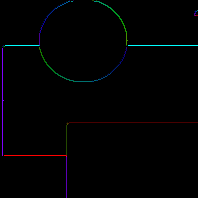
\includegraphics[width=5cm]{imgs/test/4_Affined.png} }
	\subfigure[Contour fermé]				{ 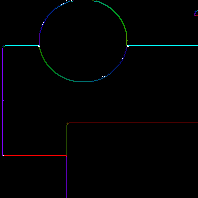
\includegraphics[width=5cm]{imgs/test/5_final.png} }
	\caption{Résultats intermédiaires pour des formes simples}
\end{figure}

\begin{figure}[ht]
	\center
	\subfigure[Gradient horizontal]				{ 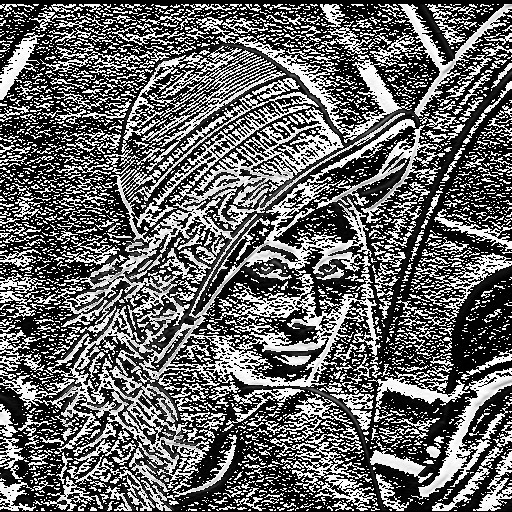
\includegraphics[width=5.5cm]{imgs/lena/1a_hGrad.png} }
	\subfigure[Gradient vertical]					{ 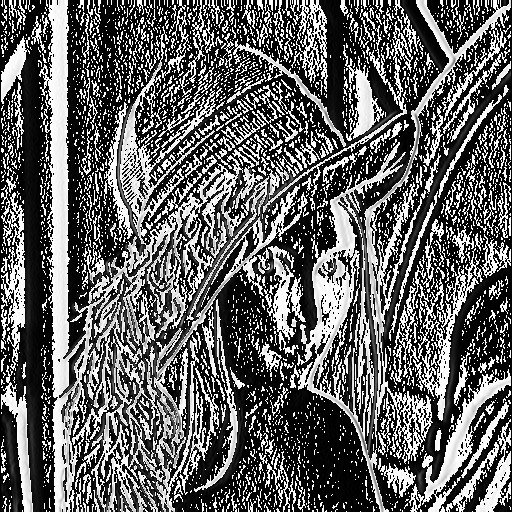
\includegraphics[width=5.5cm]{imgs/lena/1b_vGrad.png} }
	\subfigure[Gradient composé]					{ 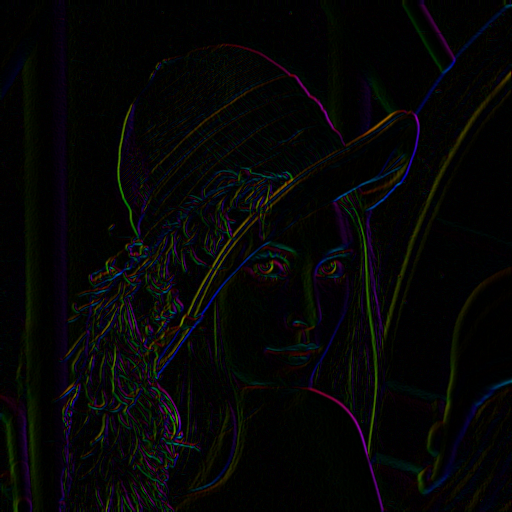
\includegraphics[width=5.5cm]{imgs/lena/2_gTone.png} }
	\subfigure[Contour seuillé]						{ 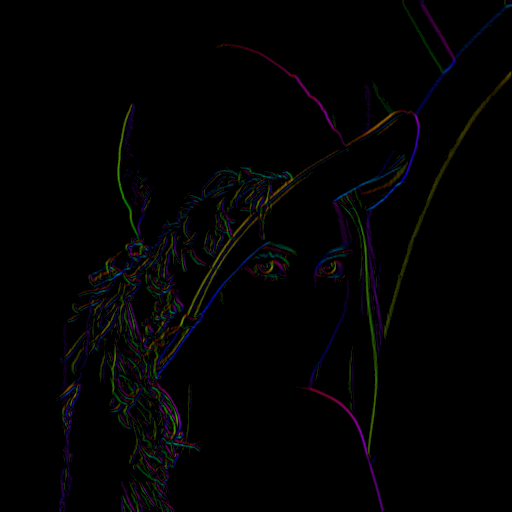
\includegraphics[width=5.5cm]{imgs/lena/3_Border.png} }	
	\subfigure[Contour affiné]						{ 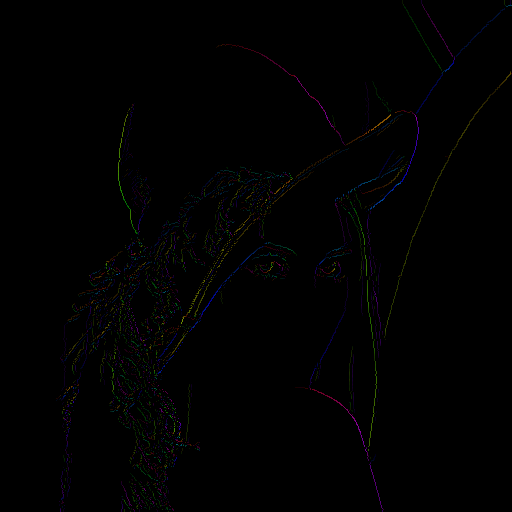
\includegraphics[width=5.5cm]{imgs/lena/4_Affined.png} }
	\subfigure[Points d'ancrage]					{ 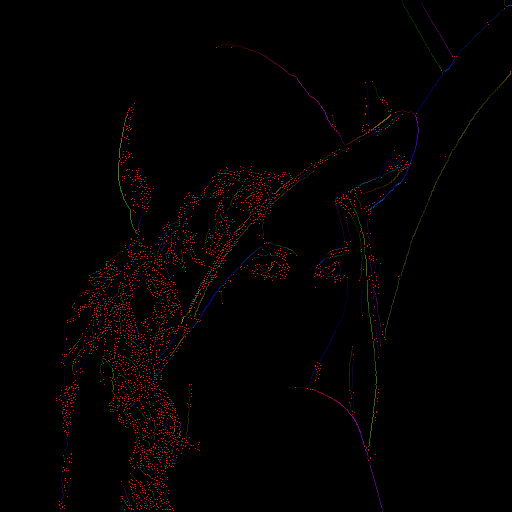
\includegraphics[width=5.5cm]{imgs/lena/5a_final_anchors.png} }
	\subfigure[Limites de la diffusion]		{ 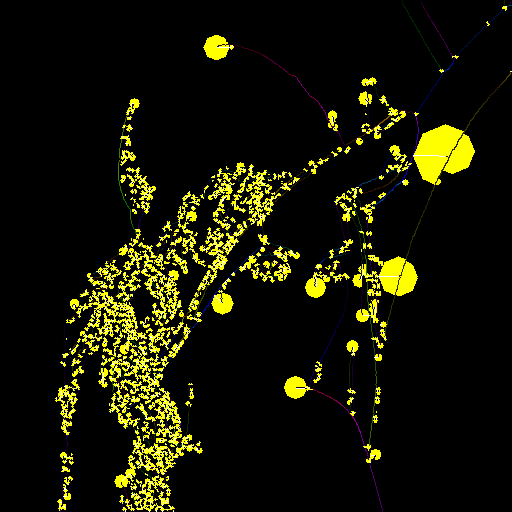
\includegraphics[width=5.5cm]{imgs/lena/5b_final_diffusion.png} }
	\subfigure[Apres fermeture]						{ 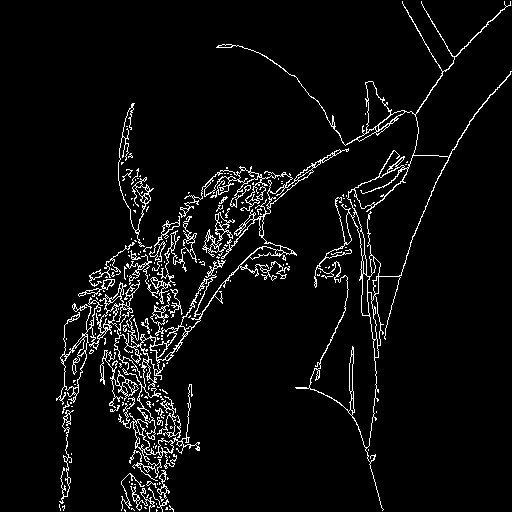
\includegraphics[width=5.5cm]{imgs/lena/5c_final_white.png} }
	\caption{Résultats intermédiaires pour Lena}
\end{figure}



\end{document}
